\documentclass{tufte-handout}

\usepackage{amsmath}
\usepackage{graphicx}
\setkeys{Gin}{width=\linewidth,totalheight=\textheight,keepaspectratio}
\usepackage{url} %% blows things up quite nicely
\usepackage{alltt}
\usepackage{semantic}
\usepackage{mcaption}
\bibliographystyle{abbrvnat}

\newtheorem{exercise}{Exercise}

\title{EECS 190 - Honors Symposium}
\author{Perry Alexander, palexand@ku.edu}
\date{Fall 2011}

\begin{document}

\maketitle

\begin{abstract}
  The object of this project is to do some very simple protocol analysis
  and design.
\end{abstract}

\begin{exercise}
  
  Figure~\ref{fig:protocol} represents a simple protocol where A and C
  are trying to communicate with B securely by establishing a shared
  secret key.  A is being honest about its identity and succeeds.  C
  is lying about its identity trying to pretend to be A.  Considering
  the protocol in figure~\ref{fig:protocol}, answer the following
  questions:

  \begin{enumerate}
  \item What is going on where ??? appears in the figure?
  \item At the end of the protocol, how do we know that A and B can
    communicate securely using N0 or N1?  This is directly related to
    the previous question.
  \item Why does C get stuck trying to establish a shared secret key?
    Why can't it pretend to be A?
  \end{enumerate}

  \begin{figure}[hbtp]
    \centering
    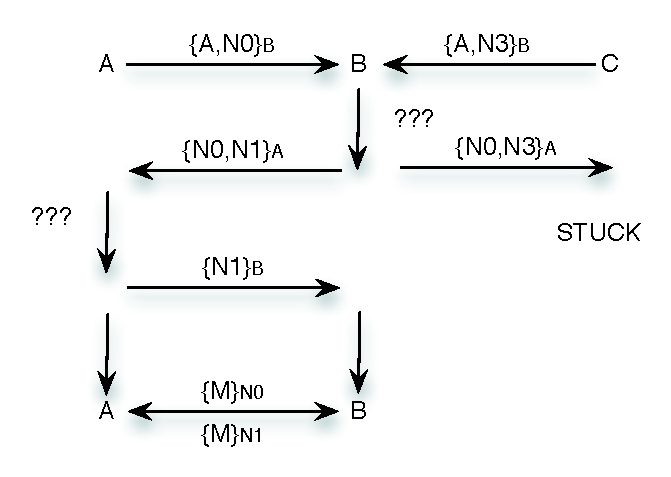
\includegraphics[width=0.75\textwidth]{protocol.pdf}
    \caption{Protocol with A and C trying to establish secure communication with B.}
    \label{fig:protocol}
  \end{figure}
\end{exercise}

\begin{exercise}

  Answer the following two questions about exchanging secure messages:
  
  \begin{enumerate}
  \item Assume A would like to send a secret message to B.  A would like to
    know that only B can read the message and B would like to know that
    only A could have sent the message.  How would you use encryption
    and signatures to accomplish this task?
  \item What would you add to your message exchange to ensure that
    someone does not grab the message A sends, store it somewhere, and
    resend it later?  (This is the tricky one.)
  \end{enumerate}  
\end{exercise}

\begin{exercise}
  There is no exercise 3.  I hated the problem I gave you and I don't
  want you to do it after all.
\end{exercise}

  
\end{document}
